
\documentclass[letterpaper,11pt]{scrartcl}
\usepackage{graphicx}
\usepackage{fullpage}

\titlehead{Guam Coconut Rhinoceros Project Technical Report}
\title{OrNV Witches Brew Experiment 1: A Last Ditch Attempt to Find Virus Pathogenetic for the Guam Cocoonut
Rhinoceros Beetle Genotype}
\author{Aubrey Moore, Ian Iriarte and Roland Quitugua}

\begin{document}

\maketitle

\begin{abstract}
Bioassays of several isolates of Oryctes nudivirus provided by AgriResearch New Zealand failed to result in 
significant pathogenicity for the Guam CRB genotype. In a 'last ditch' attempt we made a 'witches brew' slurry 
containing all frozen dead beetles from previous bioassays plus frozen virus samples in vials. Forty 
adult beetles were forced to swim in the slurry for 30 minutes on January 22, 2015. A control group of
41 beetles were forced to swim in water. Beetles were checked weekly.

By April 10, 2015, mortality of the virus treated beetles (78\%) was significantly greater than that of the
control group (54\%).
\end{abstract}

\section*{Methods}

Frozen, dead beetles from previous bioassays were added to one liter of water and made into an aqueous slurry
using a blender. Vials containing remnants of virus samples from AgResearch New Zealand were agitated in 500 ml of 
water, and this suspension was added to the blender. The slurry was poured into a small pail and
forty beetles were made to swim in this for thirty minutes. A control group of beetles was made to swim in water for 
thirty minutes.

Beetles were kept in a large container filled with moist, commercially blended steer manure and soil. 
All beetles were checked weekly. Dead beetles were recorded and frozen.

\section*{Analysis}

Data were analyzed using an IPython notebook (file name = 'OrNV'). Significance of differences in mortality
were determined using a Fisher's exact test.

\section*{Results and Discussion}

Cumulative mortality of virus-treated beetles (57\%) on April 10 (Fig. \ref{mortality}) was significantly greater than that of 
control beetles (44\%); (p = 0.0005; Fisher's exact test).
                         
It is unlikely that the beetles which died during the first two weeks of the experiment resulted from exposure
to virus, so we removed these from the experimental data and repeated the significance test. This adjustment 
did not alter the outcome: 
Mortality of virus-treated beetles (57\%) was significantly greater than that of control beetles (44\%);
(p = 0.0005; Fisher's exact test).
 
This experiment is incomplete. A postmortem will be done on the dead beetles and the 'witches brew' process
will be repeated to see if this also results in significant mortality.

% FIGURES HERE 
%%%%%%%%%%%%%%
 
\begin{figure}
\centering
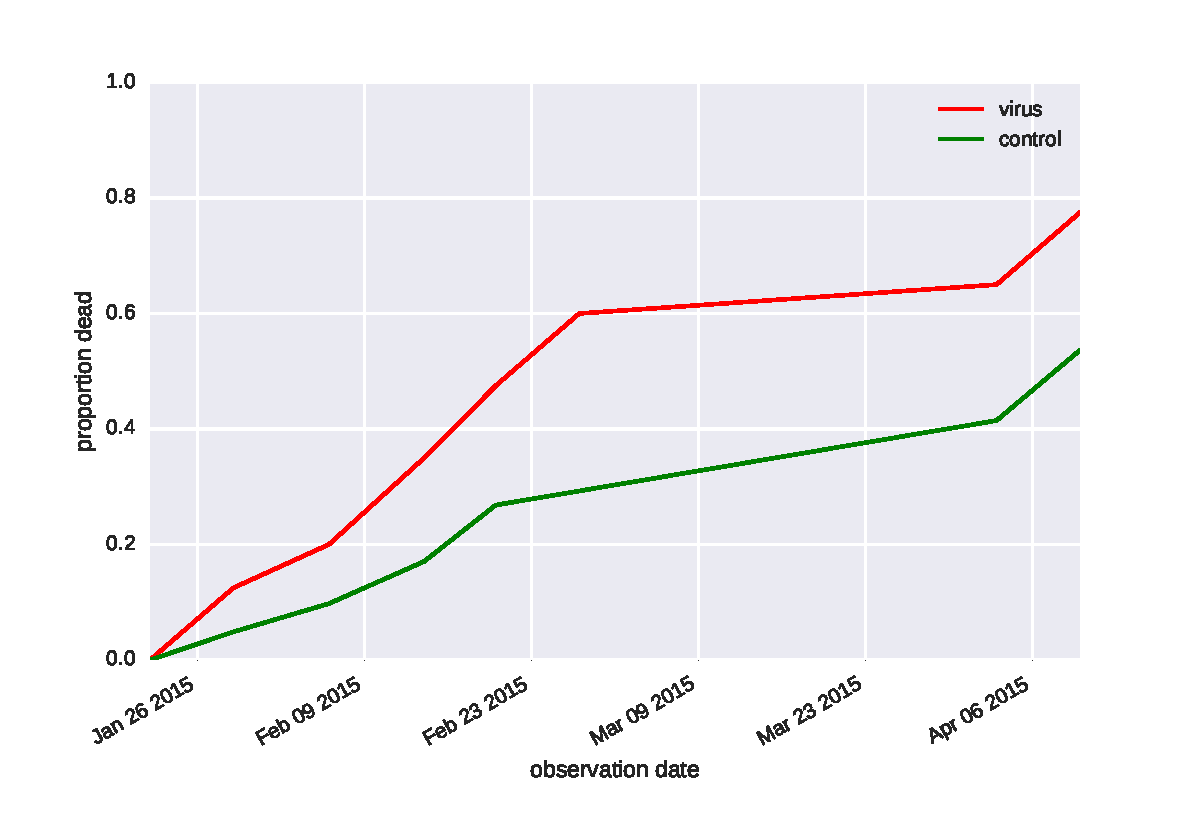
\includegraphics[width = \textwidth]{wb1_mortality.pdf}
\caption{Cumulative mortality.}
\label{mortality}
\end{figure} 
 
% END OF FIGURES
%%%%%%%%%%%%%%%%
 
%\nocite{PER-GRA_2007}
%\bibliographystyle{unsrt}
%\bibliography{ref}

\end{document}